\section{Computational spatial proteomics}


\begin{frame}{}
  \begin{center}
    \Large{Computational spatial proteomics}
  \end{center}
\end{frame}


\begin{frame}{Data analysis}
  \begin{itemize}
  \item Visualisation (cluster, unsupervised learning)
  \item Classification (supervised learning)
  \item Novelty detection (semi-supervised learning)
  \item Data integration (transfer learning)
  \item Multi-localisation (Bayesian spatial proteomics)
  \item Spatial dynamics
  \end{itemize}
  \centering
  {\Large To uncover and understand biology}
\end{frame}



\subsubsection*{Visualisation}
\label{sec:viz}

\begin{frame}{Visualisation}
  \begin{figure}
    \centering
    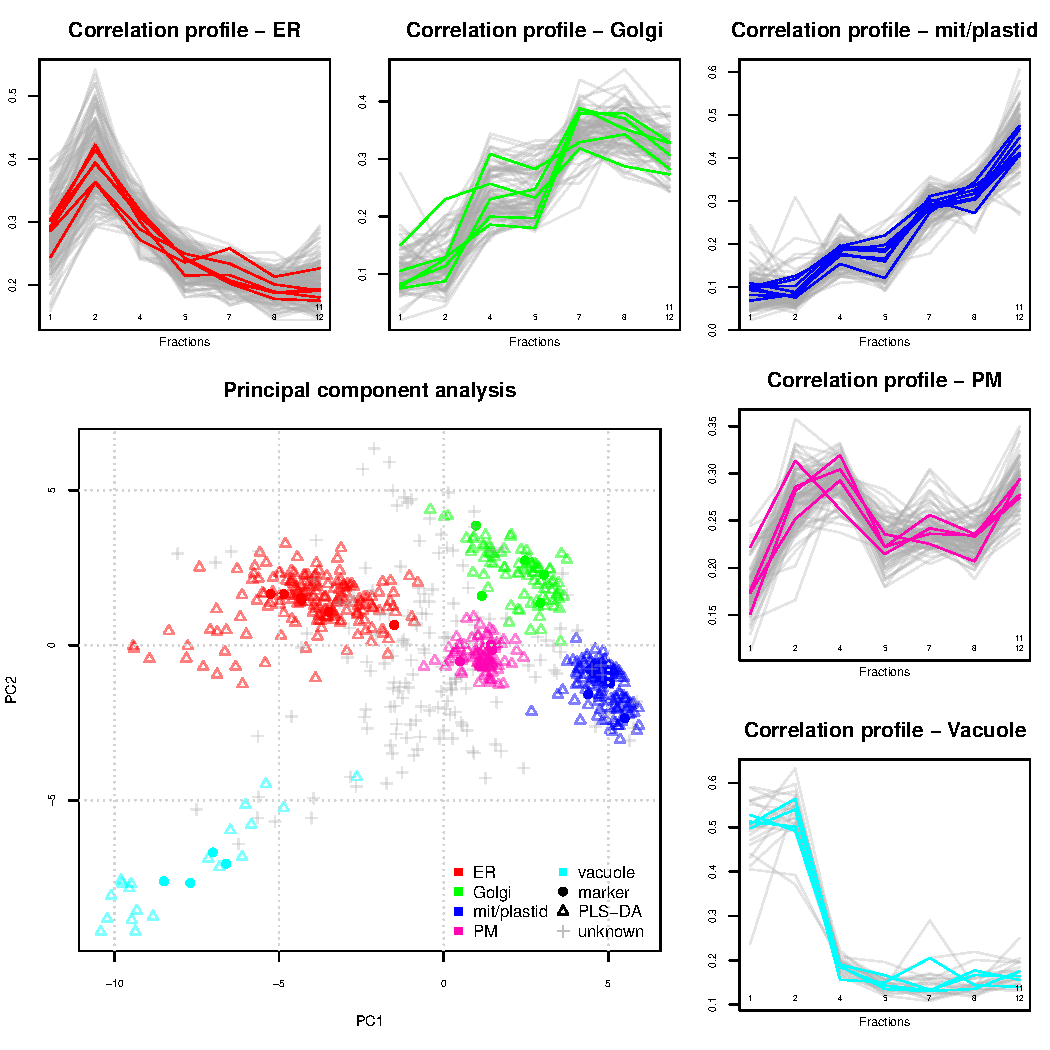
\includegraphics[width=.6\linewidth]{Figures/F04-analyses.pdf}
    \caption{From \cite{Gatto:2010}, \textit{Arabidopsis thaliana} data
      from \cite{Dunkley:2006}}
  \end{figure}
\end{frame}

\subsubsection*{Machine learning}
\label{sec:ml}

\begin{frame}{Supervised Machine Learning}
  \begin{figure}[h]
    \centering
    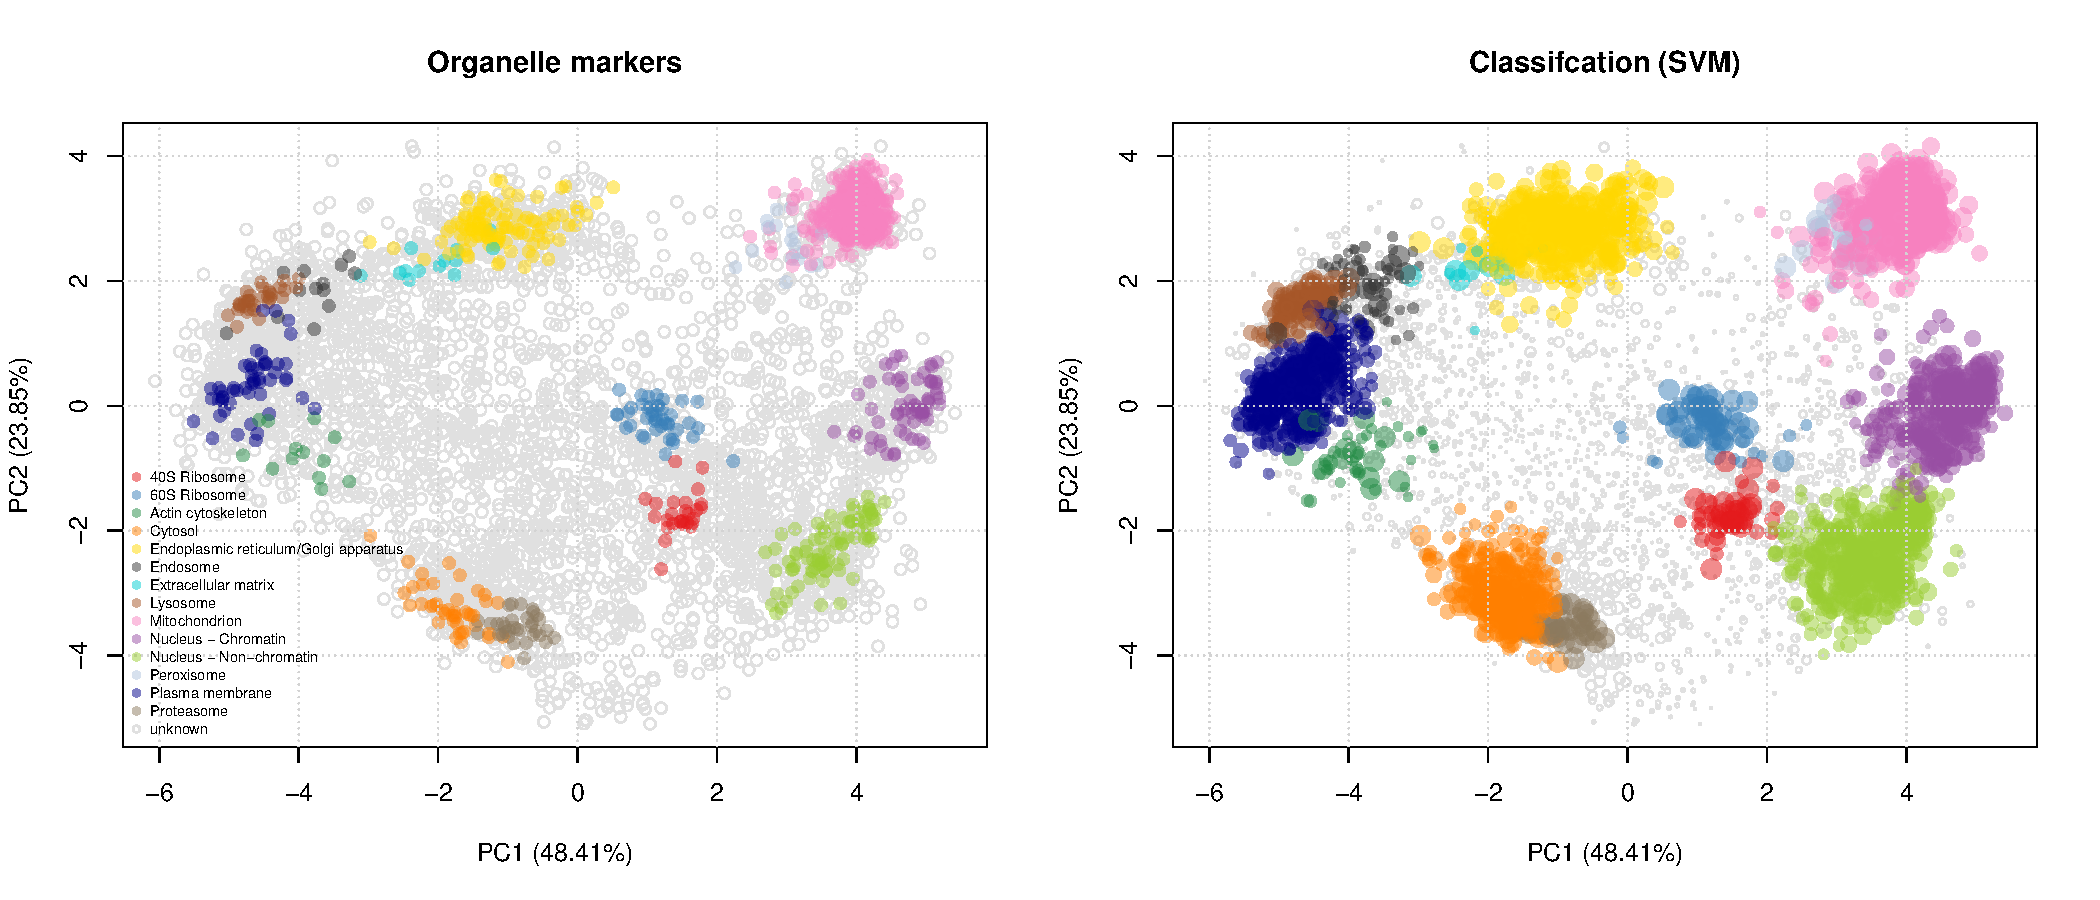
\includegraphics[width=\linewidth]{figs_local/hyperlopit-class.pdf}
    \caption{Support vector machines classifier (after 5\% FDR
      classification cutoff) on the embryonic stem cell data from
      \cite{Christoforou:2016}.}
  \end{figure}
\end{frame}


\begin{frame}{}
  \begin{center}
    \Large{Novel \textbf{computational biology research and developments}
    to acquire reliable biological knowledge.}
  \end{center}
\end{frame}

\subsection{Novelty detection}

\begin{frame}{Importance of annotation}

  \begin{columns}[t]
    \begin{column}[T]{0.43\textwidth}
      \begin{centering}
        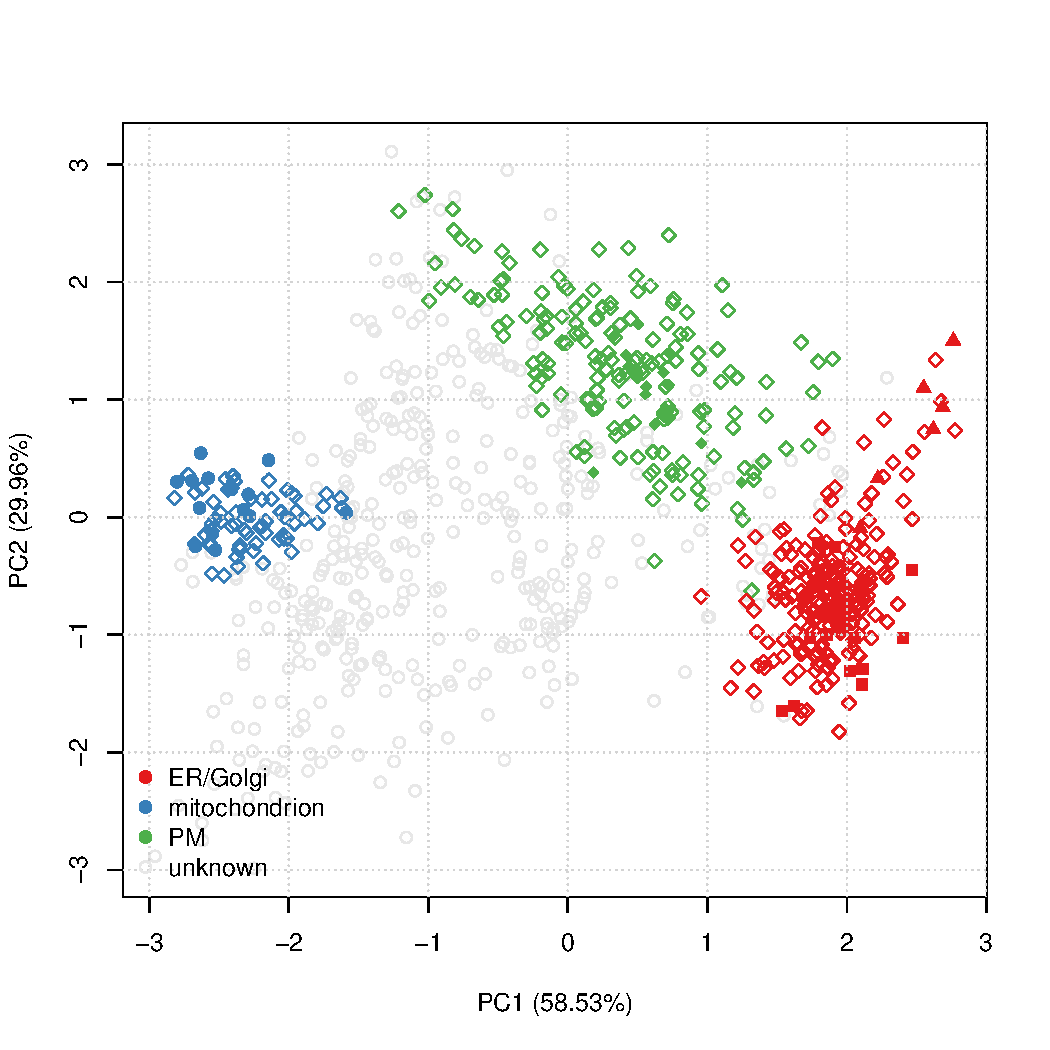
\includegraphics[width=1\linewidth]{Figures/tan2009r1org.pdf}
      \end{centering}
    \end{column}
    \begin{column}[T]{0.56\textwidth}
      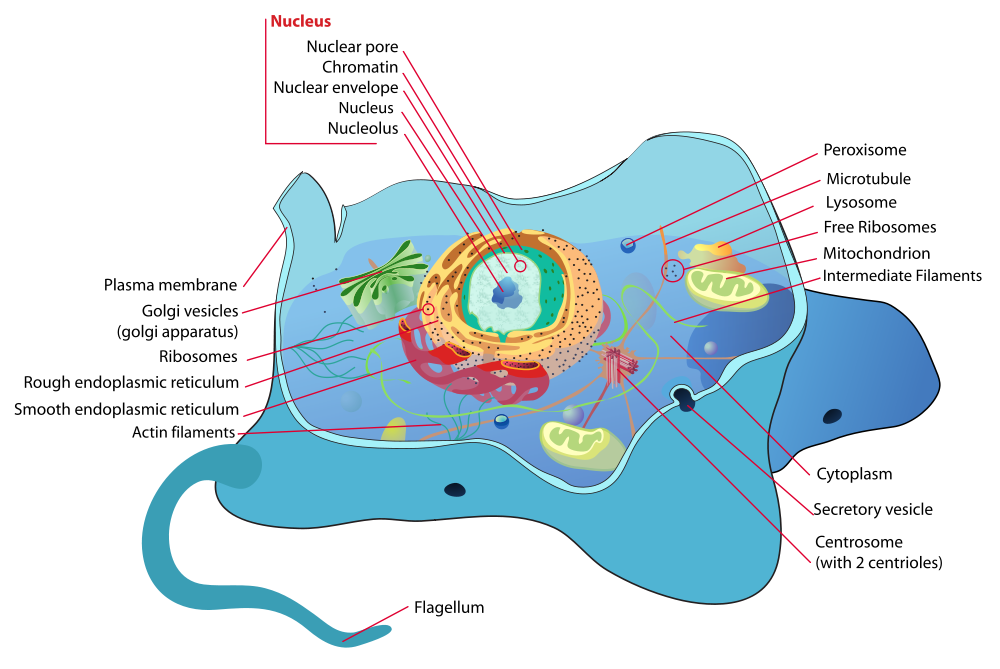
\includegraphics[width=1\linewidth]{Figures/Animal_cell_structure.png}
    \end{column}
  \end{columns}
  Incomplete annotation, and therefore lack of training data, for
  many/most organelles. \textit{Drosophila} data from \cite{Tan2009}.
\end{frame}

\begin{frame}{Semi-supervised learning: novelty detection}
  \begin{figure}
    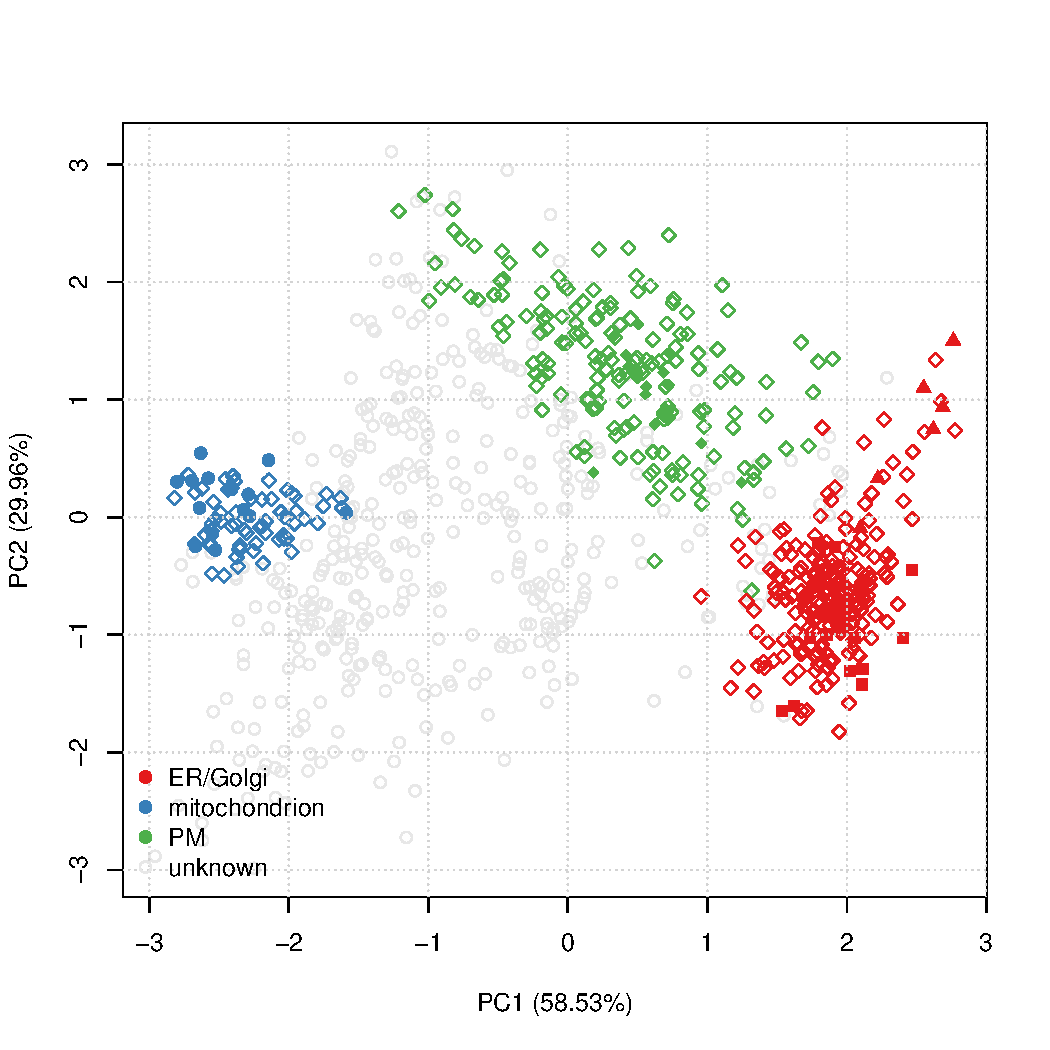
\includegraphics[width=.48\linewidth]{Figures/tan2009r1org.pdf}
    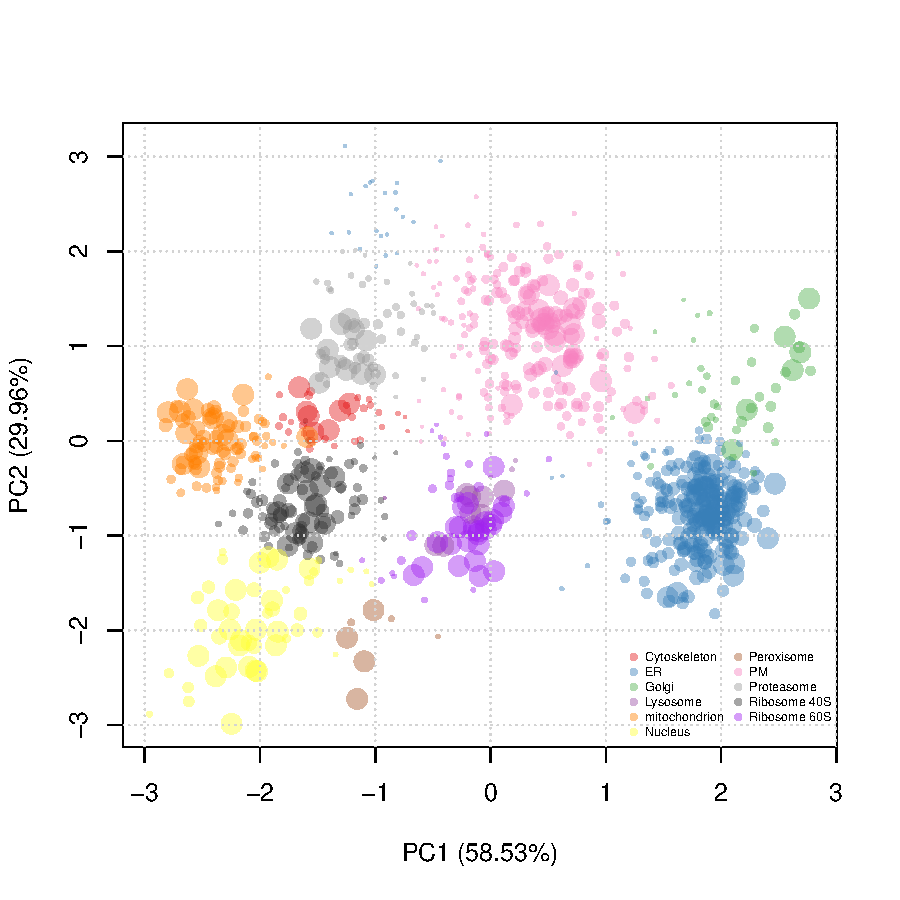
\includegraphics[width=.5\linewidth]{Figures/pdres2fig.pdf}
    \caption{Left: Original \textit{Drosophila} data from
      \cite{Tan2009}. Right: After semi-supervised learning and
      classification, \cite{Breckels:2013}.}
  \end{figure}
\end{frame}

% \begin{frame}
%   \centering
%   \begin{columns}[t]
%     \begin{column}[T]{0.4\textwidth}
%       \begin{figure}[h]
%         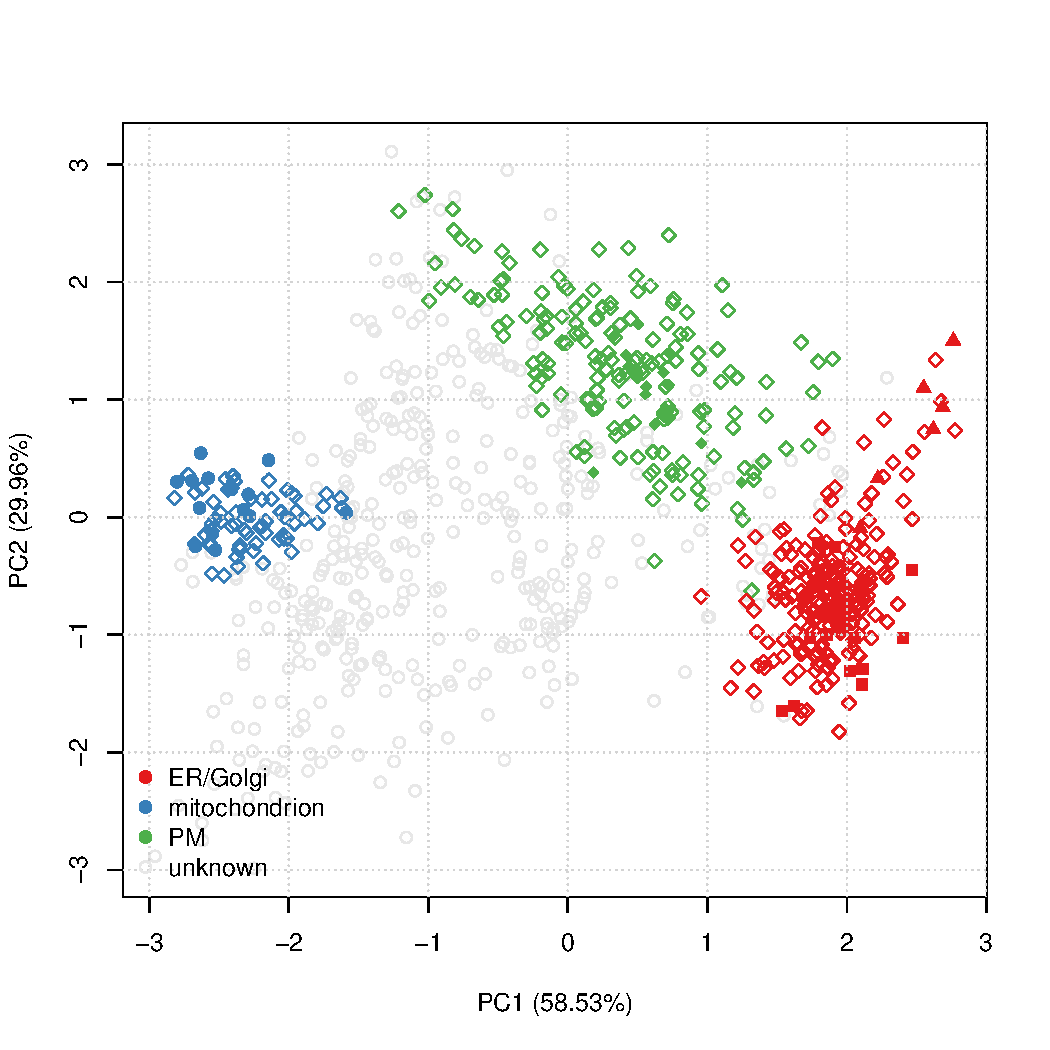
\includegraphics[width=.9\linewidth]{Figures/tan2009r1org.pdf} \\
%         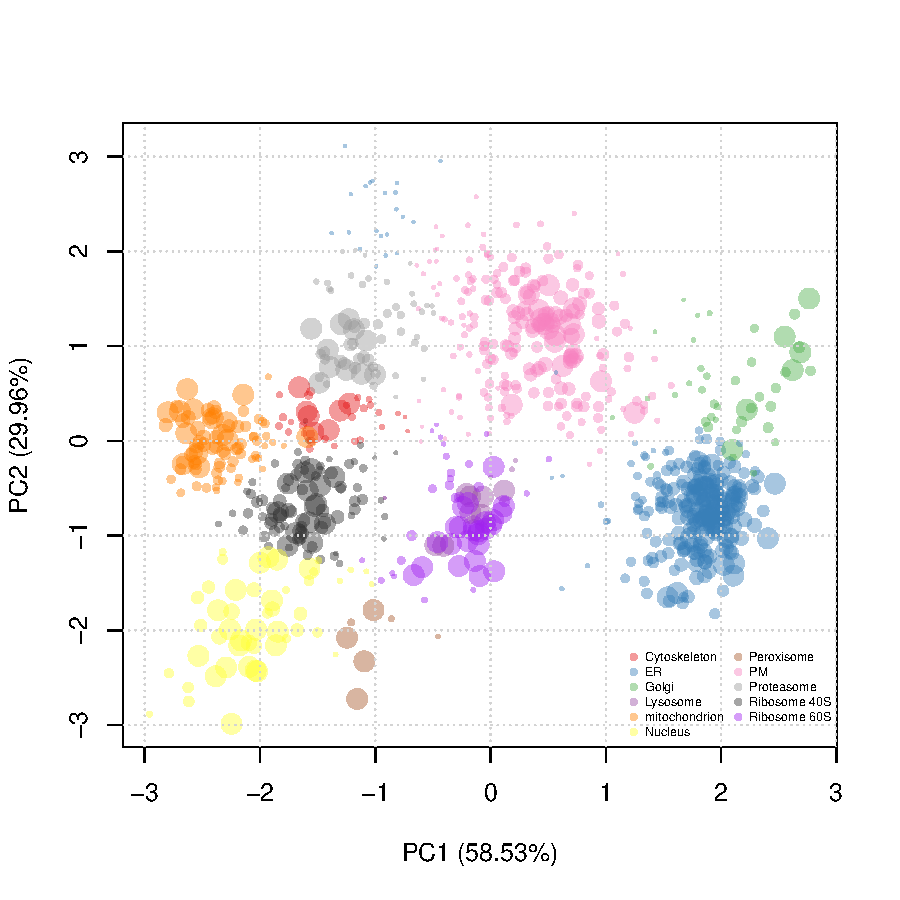
\includegraphics[width=.9\linewidth]{Figures/pdres2fig.pdf}
%       \end{figure}
%     \end{column}
%     \begin{column}[T]{0.59\textwidth}
%       \begin{figure}[h]
%         \includegraphics[width=.9\linewidth]{Figures/phenodisco.pdf}
%       \end{figure}
%     \end{column}
%   \end{columns}
%   % \caption{The \texttt{phenoDisco} algorithm \citep{Breckels:2013}.}
% \end{frame}

%% \subsection{Improving on LOPIT}

%% \begin{frame}{Improving on LOPIT}

%%   Improving is obtaining better \textbf{sub-cellular resolution} to
%%   increase the number of protein that can be \textbf{confidently}
%%   assigned to a sub-cellular niche $\Rightarrow$ \textbf{biological
%%     discoveries}.

%%   \begin{figure}[h]
%%     \centering
%%     \includegraphics[width=1\linewidth]{./Figures/E14-lopit-hyperlopit.pdf}
%%     \caption{E14TG2a embryonic stem cells: old (left, published in
%%       \cite{Breckels:2013}) \textit{vs.} new, better resolved (right)
%%       experiments (\cite{Christoforou:2016}).}
%%   \end{figure}

%% \end{frame}

%% \begin{frame}{Improving on LOPIT}


%%   \centering
%%   \begin{tabular}{| p{5cm} | p{5cm} |}
%%     \hline
%%     \makecell{LOPIT\\ \cite{Dunkley:2006} \\ \cite{Gatto:2014}}    & \makecell{\textbf{Computational}:\\ \textit{transfer learning}\\ \cite{Breckels:2016}} \\
%%     \hline
%%     \makecell{\textbf{Experimental}:\\ \textit{hyperLOPIT}\\ \cite{Christoforou:2016} \\ \cite{Mulvey:2017} \\ \cite{Breckels:2016b}} & \makecell{\textbf{Biological}\\\textbf{discoveries}}  \\
%%     \hline
%%   \end{tabular}
%% \end{frame}

%% \subsubsection{Experimental advances: hyperLOPIT }

%% \begin{frame}{Experimental advances: hyperLOPIT \cite{Christoforou:2016}}
%%   \begin{figure}[h]
%%     \centering
%%     \includegraphics[width=.7\linewidth]{./Figures/nprot-hyperlopit-2017-026-F1.jpg}
%%     \caption{From \cite{Mulvey:2017} \textit{Using \textbf{hyperLOPIT}
%%         to perform high-resolution mapping of the spatial proteome}:
%%       (1) organelle separation and enrichment by \textbf{density
%%         gradient ultracentrifugation}, (2) \textbf{chromatin and
%%         cytosol} enrichment fractions, and (3) accurate quantification
%%       using \textbf{synchronous precursor selection (SPS)-MS$^3$ for
%%         TMT 11-plex} quantification.}
%%     \label{fig:hyperlopit}
%%   \end{figure}
%% \end{frame}

%% \begin{frame}
%%   \begin{figure}[h]
%%     \centering
%%     \includegraphics[width=1\linewidth]{./Figures/E14-lopit-hyperlopit-rep1.pdf}
%%     \caption{E14TG2a LOPIT on 8 fractions (using iTRAQ 8-plex) and
%%       1109 proteins \textit{vs.}  hyperLOPIT on 10 fractions (using
%%       TMT 11-plex) and SPS-MS$^3$ for 5032 proteins.}
%%   \end{figure}

%% \end{frame}

\subsection{Computational advances: Transfer learning}

\begin{frame}{Computational advances: Transfer learning}
  What about using \textbf{addition data}, such as annotations from
  the Gene Ontology (GO), sequence features (pseudo aminoacid
  composition), signal peptide, trans-membrane domains (length,
  number, ...), images (IF, FP), interaction data, prediction
  software, \ldots

  \begin{block}{}
    \begin{itemize}
    \item From a \underline{user perspective}: \textbf{"free/cheap"}
      vs. expensive and time-consuming experiments.
    \item Abundant (all proteins, 100s of features) vs. (experimentally)
      limited/\textbf{targeted} (1000s of proteins, 6 -- 20 of features)
    \item For localisation in \underline{system at hand}: \textit{low}
      vs. high \textbf{quality}
    \item \textbf{Static} vs. \textbf{dynamic}
    \end{itemize}
  \end{block}

\end{frame}

\begin{frame}{}

  \begin{block}{Transfer learning}
    Support/complement the \textbf{primary} target domain
    (experimental data) with \textbf{auxiliary} data (annotation,
    imaging, PPI, ...)  features without compromising the integrity of
    our primary data.
  \end{block}

\end{frame}


\begin{frame}
  \begin{center}
    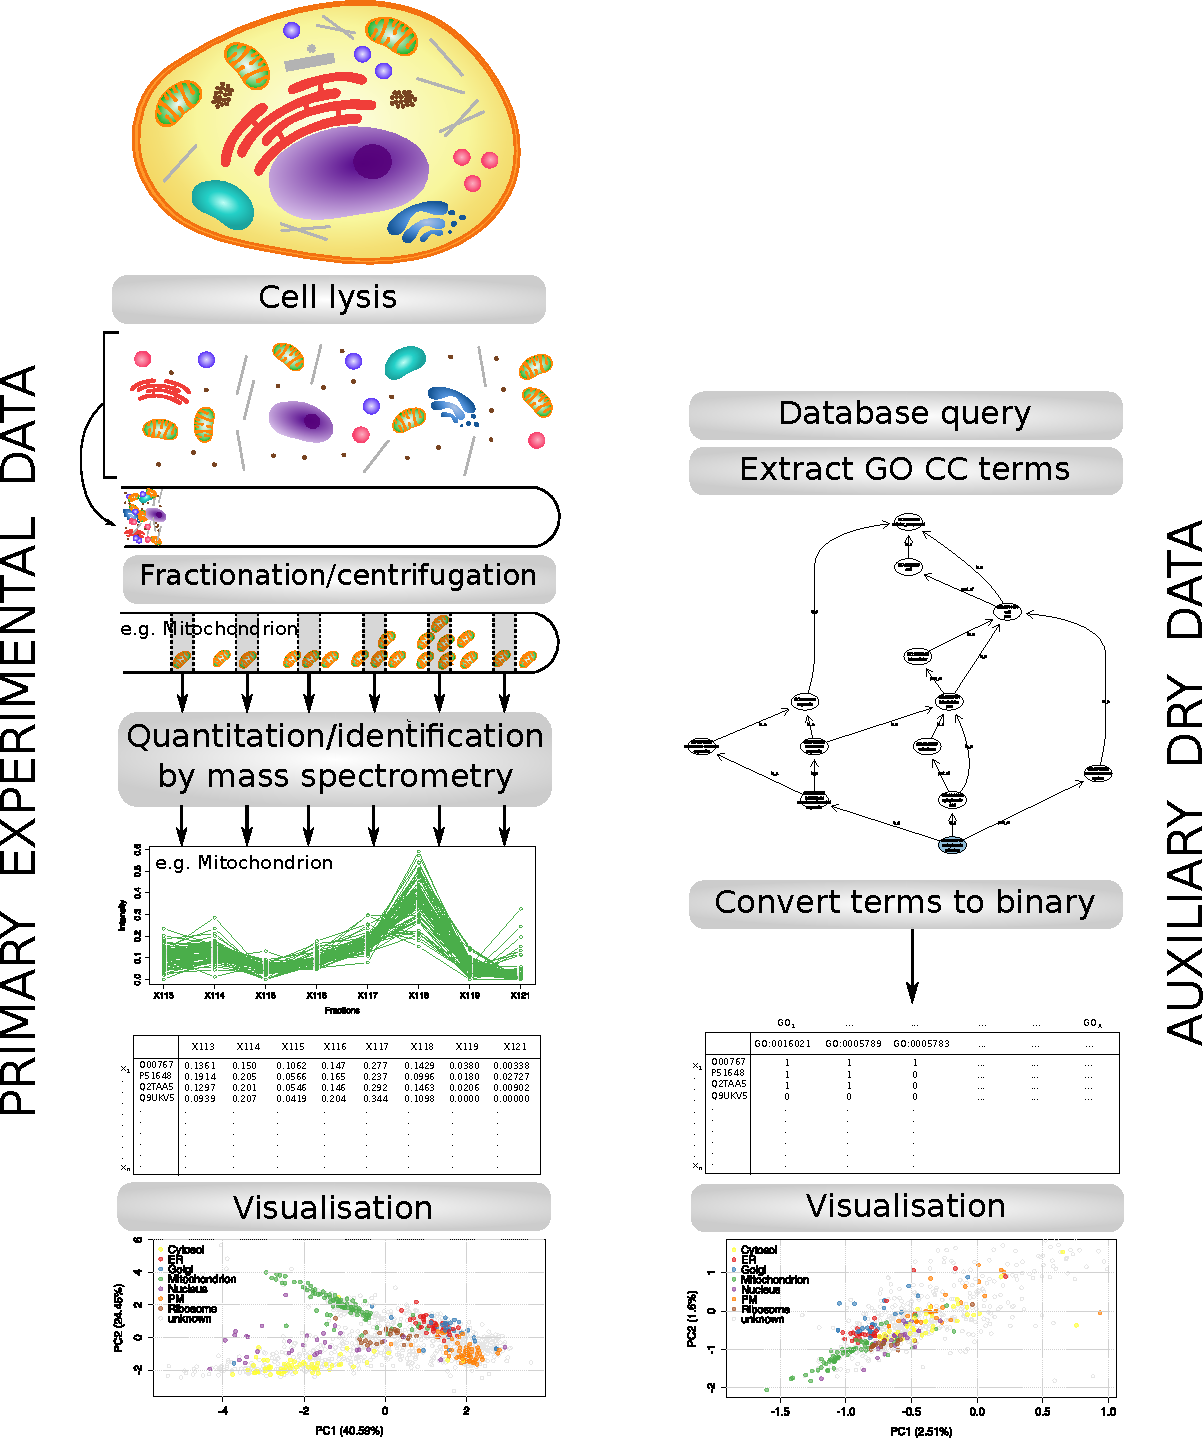
\includegraphics[width=.7\linewidth]{figures/workflow.pdf}
  \end{center}
\end{frame}


\begin{frame}{Transfer learning results}

  \begin{figure}[h]
    \centering
    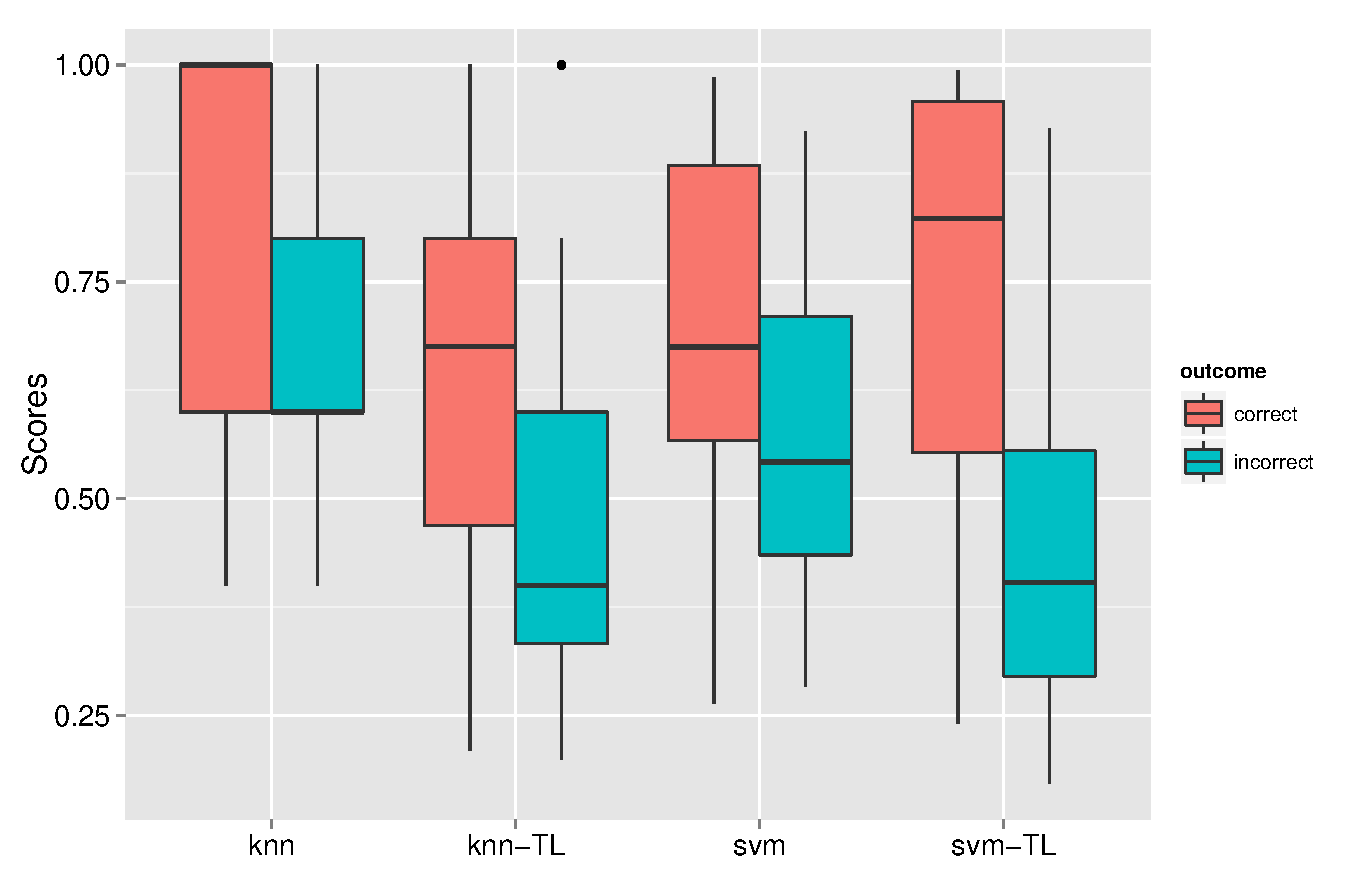
\includegraphics[width=.8\linewidth]{./Figures/2016-PLoSCB-TL-classifierDiscriminationPowerk5.pdf}
    \caption{{\footnotesize From \cite{Breckels:2016} \textit{Learning from
          heterogeneous data sources: an application in spatial
          proteomics}.}
    }
\label{fig:tlres}
  \end{figure}

\end{frame}

\subsection{Embracing uncertainty}

\begin{frame}{A Bayesian Mixture Modelling Approach For Spatial Proteomics}

  \begin{itemize}

    \item<+-> \textit{T Augmented Gaussian Mixture model (TAGM)} is a
      \textbf{multivariate Gaussian generative model} for MS-based
      spatial proteomics data. It posits that each annotated
      sub-cellular niche can be modelled by a multivariate Gaussian
      distribution.

    \item<+-> With the prior knowledge that many proteins are not
      captured by known sub-cellular niches, we augment our model with
      an \textbf{outlier component}. Outliers are often dispersed and
      thus this additional component is described by a heavy-tailed
      distribution: the multivariate Student's t-distribution, leading
      us to a \textit{T Augmented Gaussian Mixture model}.

    \item<+-> This methodology allows proteome-wide
      \textbf{uncertainty quantification} (Shannon entropy), thus
      adding a further layer to the analysis of spatial proteomics.

  \end{itemize}
\end{frame}

\begin{frame}[fragile]{}
      \begin{figure}
        \sidebysidecaption{0.65\linewidth}{0.3\linewidth}{
          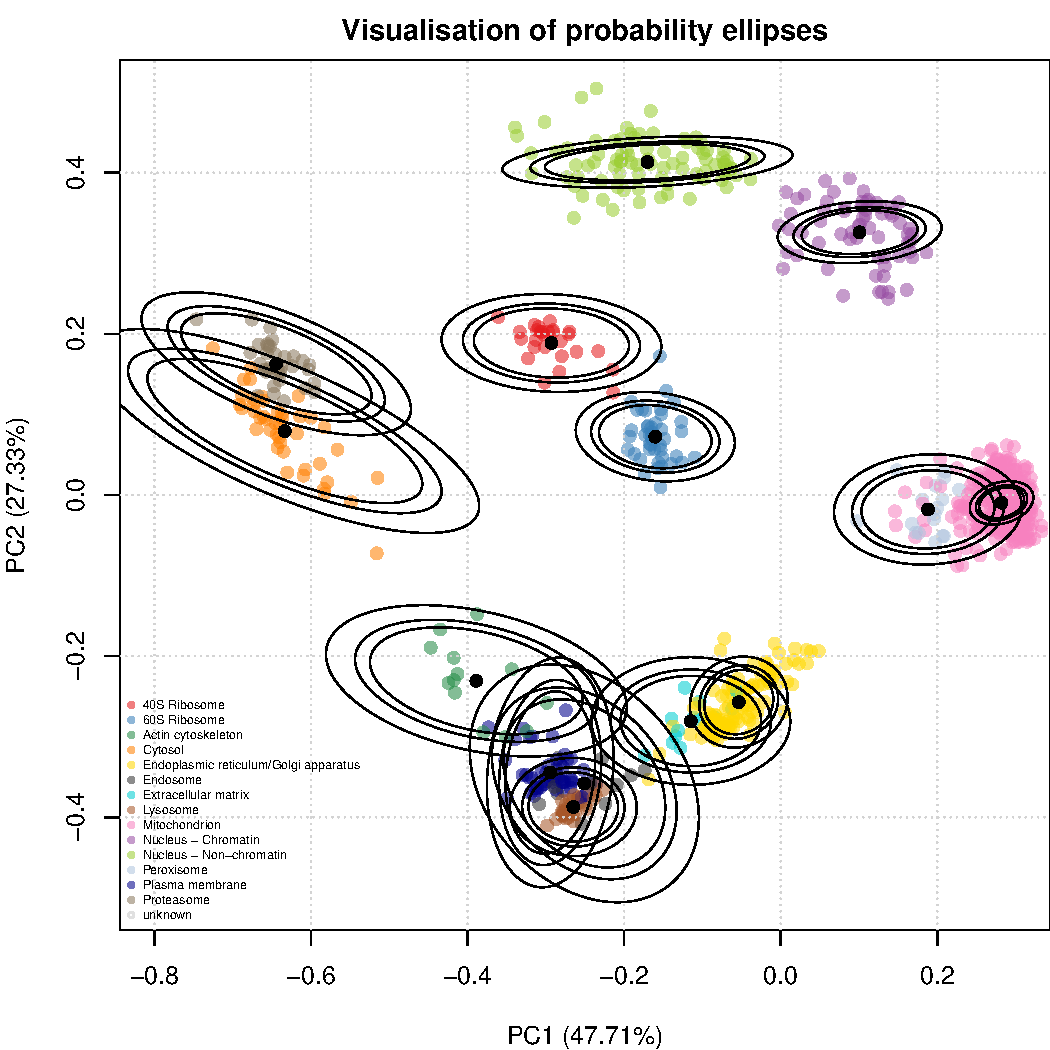
\includegraphics[width=1\linewidth]{./figs_local/pca12-ellipses-1.pdf}
        }{
          \caption{\scriptsize \justifying Illustration of how the
            TAGM model describes the pluripotent mouse embryonic stem
            cell data. Each ellipse contains a proportion of total
            probability of a particular multivariate Gaussian density.
            The outer ellipse contains $99\%$ of the total probability
            whilst the middle and inner ellipses contain $95\%$ and
            $90\%$ of the probability respectively.}
          \label{fig:tagm}
        }
      \end{figure}

      %% NOTE that while some sub-cellular clusters overlap along PC1 and
      %% PC2, they are separated along additional dimensions.

\end{frame}

\begin{frame}{}
      \begin{figure}
        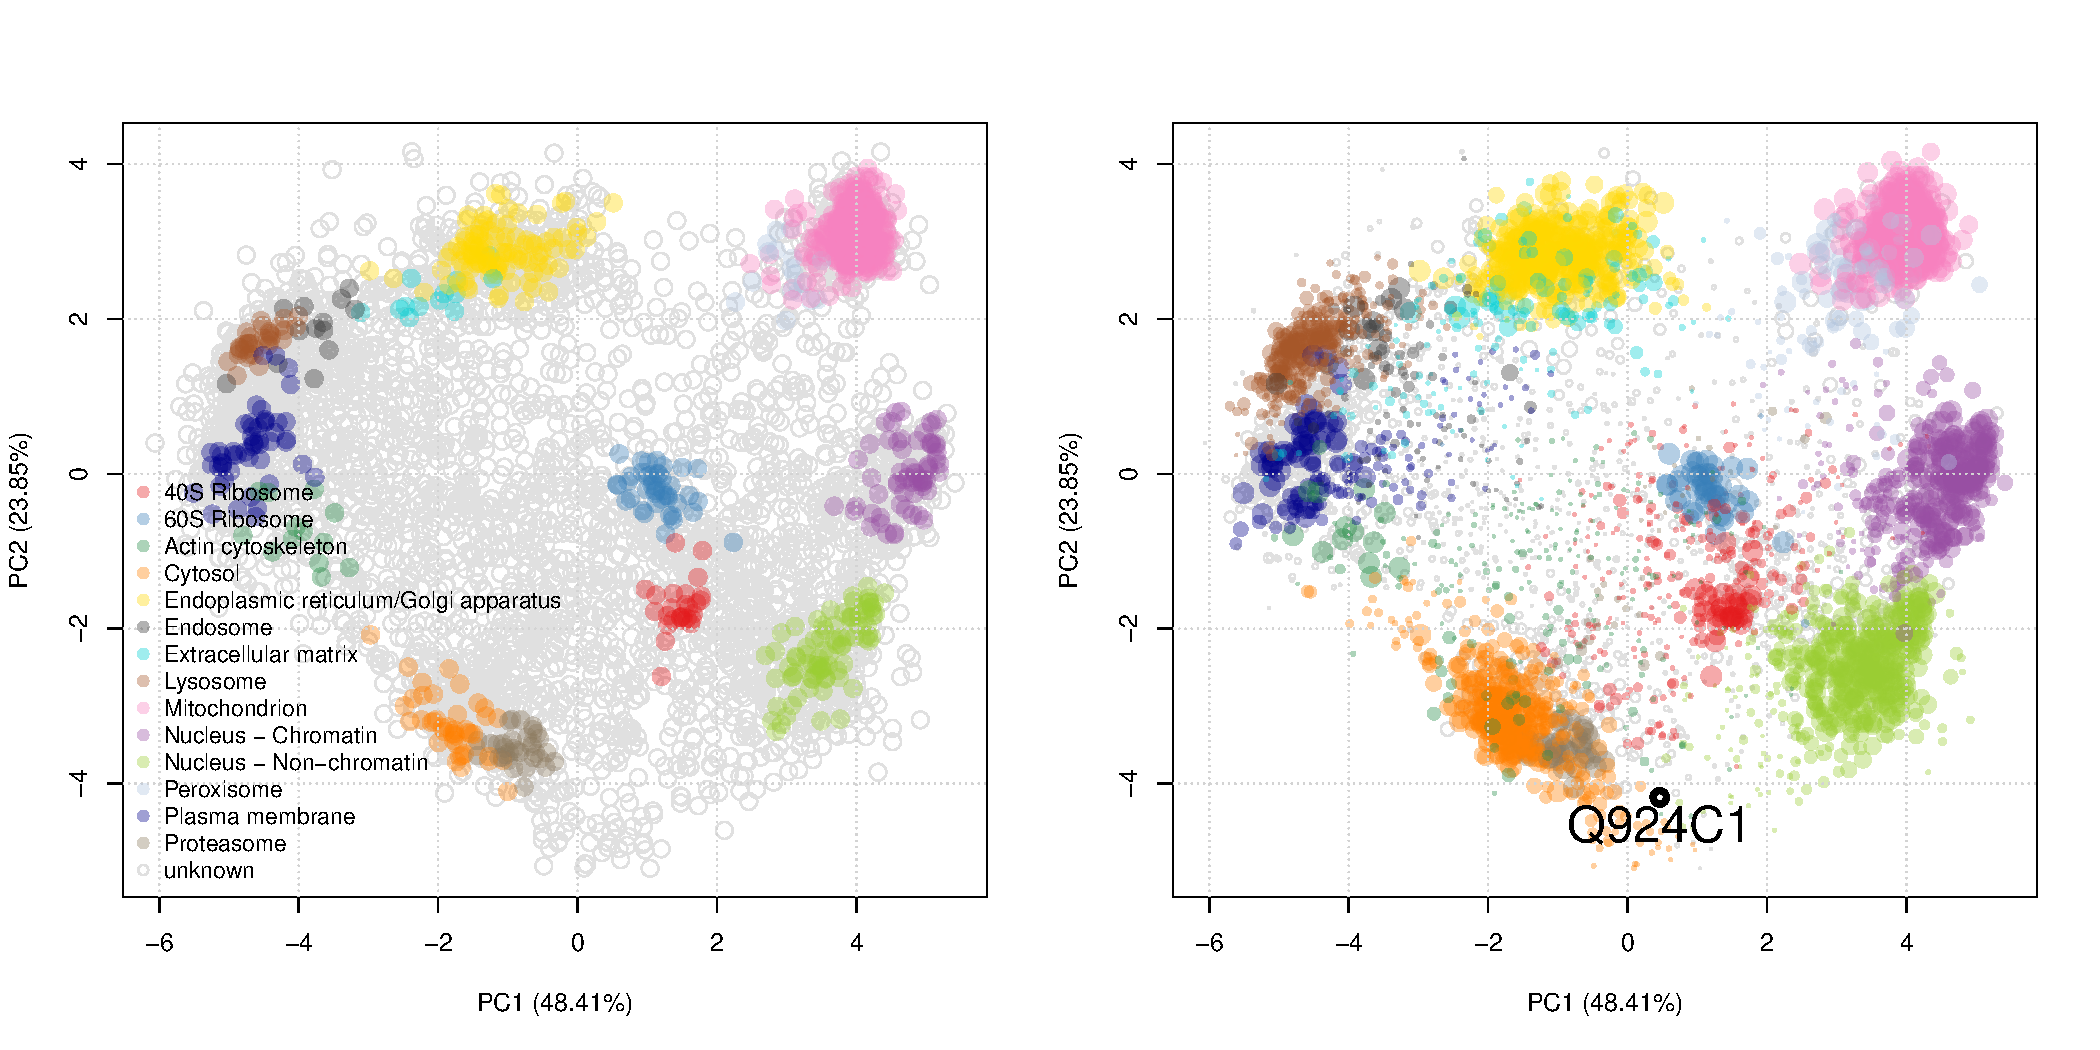
\includegraphics[width=1\linewidth]{./figs_local/pca.pdf}
        \caption{Assignment of proteins of
          \textit{unknown} location to one of the annotated
          classes. The dots are scaled according to the protein
          assignment probabilities.}
      \end{figure}
\end{frame}

\begin{frame}{}
  \begin{figure}
    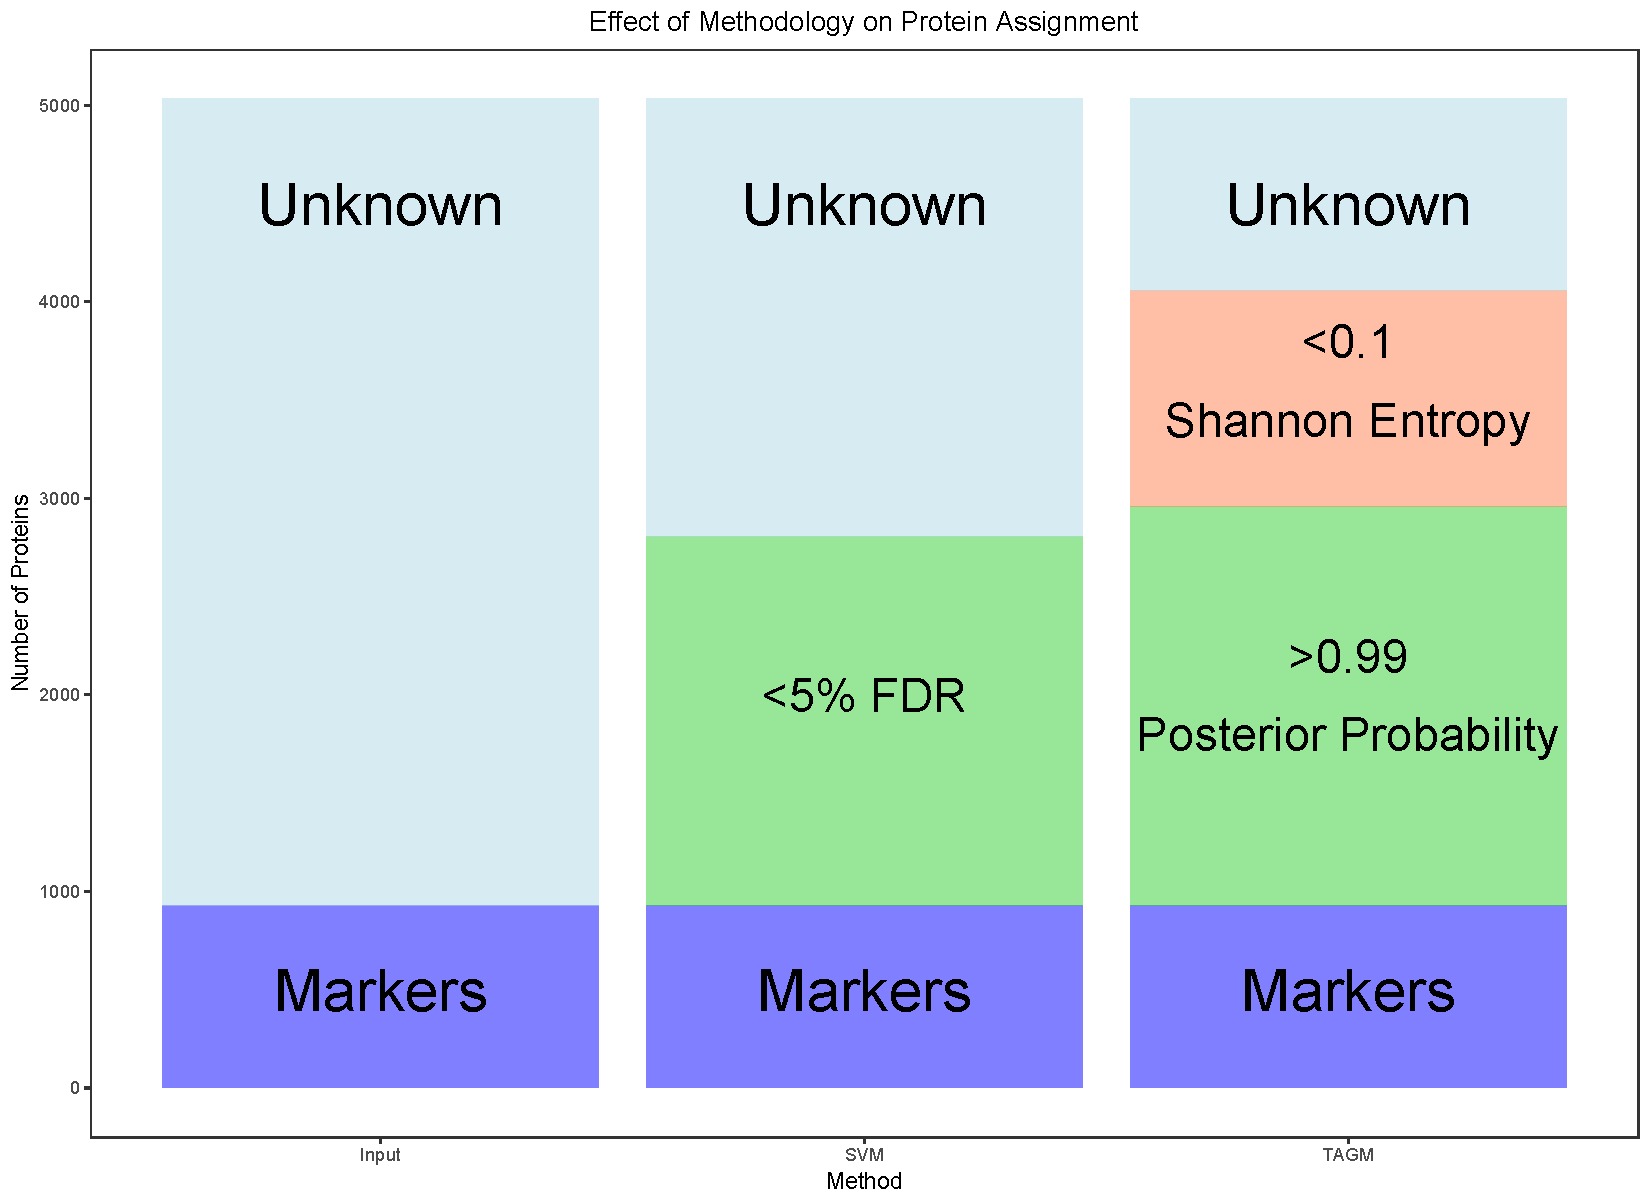
\includegraphics[width=.8\linewidth]{./figs_local/ConcludePlot.pdf}
  \end{figure}
\end{frame}

\begin{frame}
  \begin{figure}
    \centering
    \sidebysidecaption{0.55\linewidth}{0.42\linewidth}{
      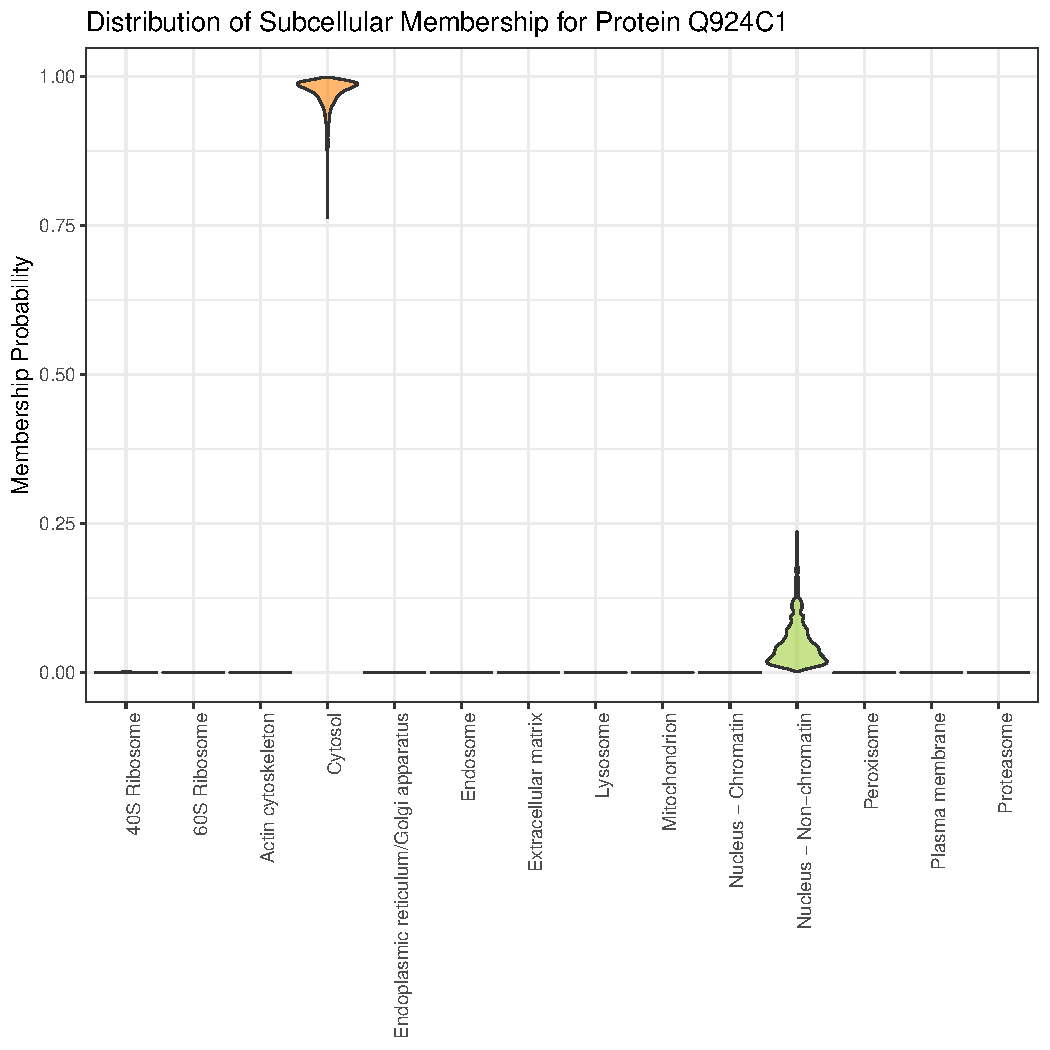
\includegraphics[width=1\linewidth]{./figs_local/Q924C1-prob-1.pdf}
    }{
    \caption{\scriptsize \justifying Exportin 5 (Q924C1) forms part of
      the micro-RNA export machinery, transporting miRNA from the
      nucleus to the cytoplasm for further processing.  It then
      translocates back through the nuclear pore complex to return to
      the nucleus to mediate further transport between nucleus and
      cytoplasm. The model correctly infers that it most likely
      localises to the cytosol but there is some uncertainty with this
      assignment. This uncertainty is reflected in possible assignment
      of Exportin 5 to the nucleus non-chromatin and reflects the
      multi-location of the protein.}  }
    %% NOTE SVM failed to classify exportin 5 to any of the two
    %% biologically plausible locations, arguably due to the similarity
    %% of the cytosol and peroxysome, to which it got assigned.

  \end{figure}
\end{frame}


\begin{frame}{Whole sub-cellular proteome uncertainty}
  \begin{figure}
    \centering
    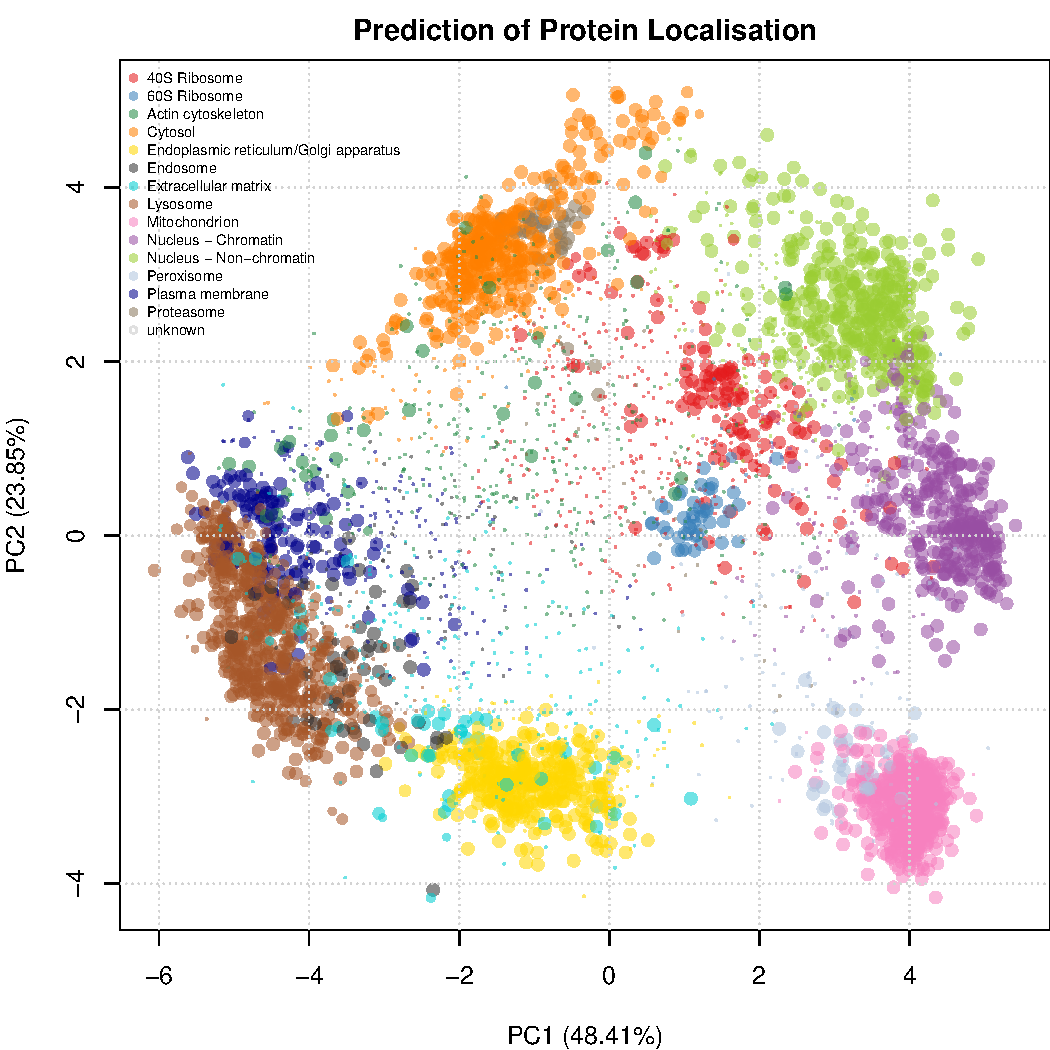
\includegraphics[width=.32\linewidth]{./figs_local/pca-tagm-mcmc-1.pdf}
    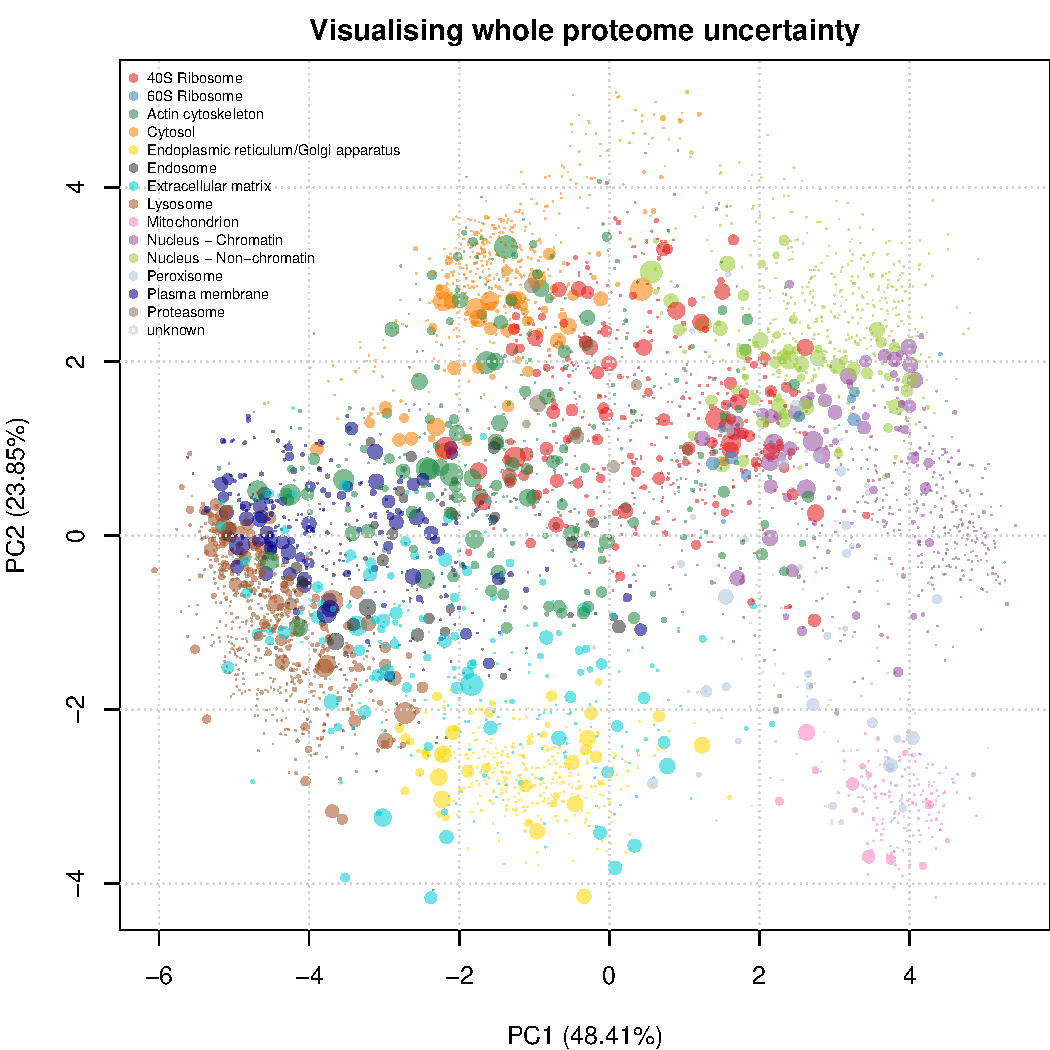
\includegraphics[width=.32\linewidth]{./figs_local/pca-tagm-map-1.pdf}
    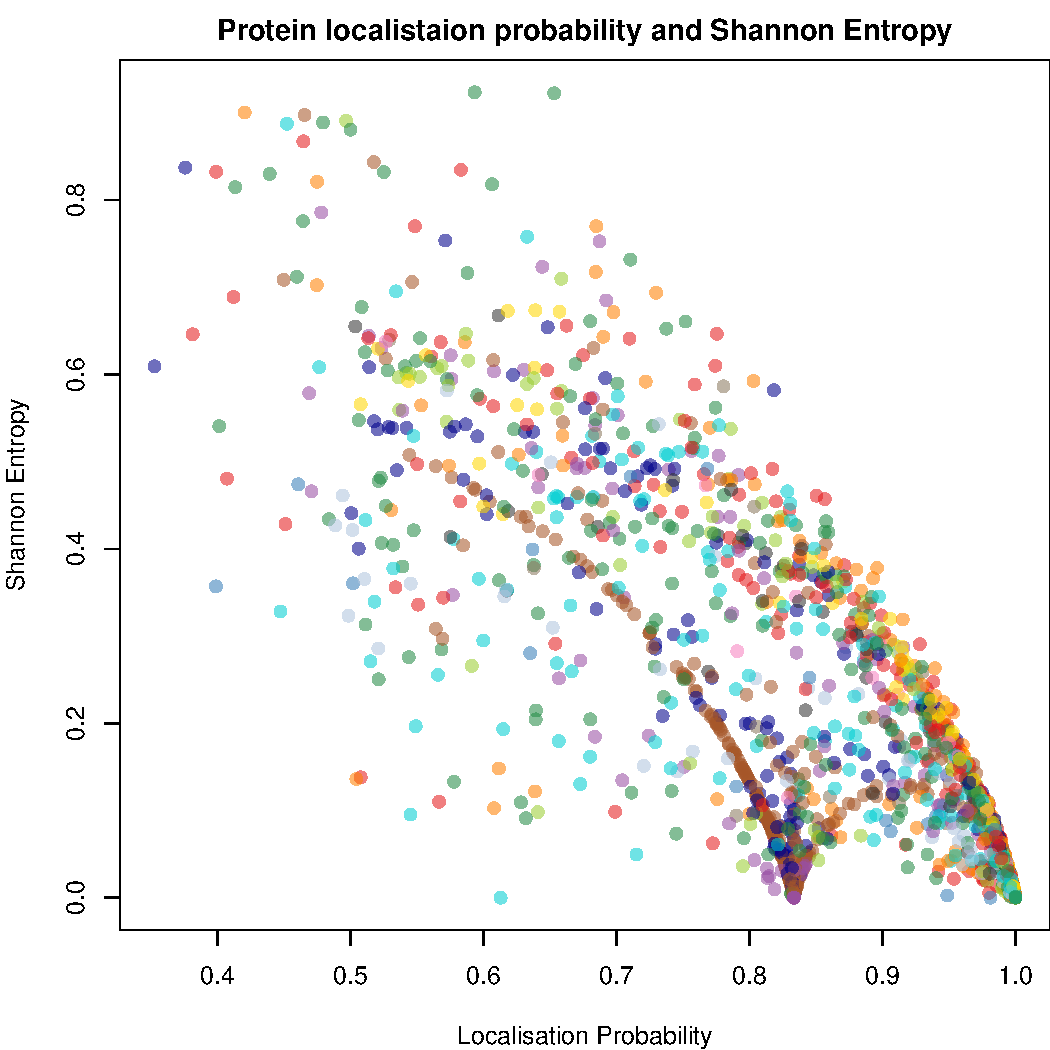
\includegraphics[width=.32\linewidth]{./figs_local/prob-vs-shannon-1.pdf}
  \end{figure}
\end{frame}



%% \subsubsection{Dual-localisation}

%% \begin{frame}
%%   \textcolor{Blue}{\textbf{Dual-localisation}} Proteins may be present
%%   simultaneously in several organelles (e.g. trafficking). Simulation
%%   on \textit{A. thaliana} data from \cite{Dunkley:2006}
%%   \citep{Gatto:2014a} (left). Example from embryonic stem cells
%%   \citep{Christoforou:2016} (right).
%%   \begin{columns}
%%     \begin{column}{.5\textwidth}
%%       \includegraphics[width=1\linewidth]{figures/dual-loc.pdf}<+->
%%     \end{column}
%%     \begin{column}{.5\textwidth}<+->
%%       \centering
%%       \includegraphics[width=.8\linewidth]{figures/Tfe3.png}\\
%%       \tiny From \cite{Betschinger:2013} \\
%%       \includegraphics[width=1\linewidth]{figures/Tfe3.pdf}
%%     \end{column}
%%   \end{columns}
%% \end{frame}

\subsection{Spatial dynamics}

\begin{frame}{Spatial dynamics}
  \begin{block}{Trans-localisation event during monocyte to macrophage
      differentiation}
    Investigate the effect of lipopolysaccharides (LPS)-mediated
    inflammatory response in human monocytic cells (THP-1)
  \end{block}

  \begin{block}{Data}
    \begin{itemize}
    \item Triplicate \textbf{temporal} profiling (0, 2, 4, 6, 12, 24
      hours).
    \item Triplicate \textbf{spatial} profiling (0 vs 12 hours) -
      early trafficking, before actual morphological differentiation
      at 24h.
    \end{itemize}
  \end{block}

  Work lead by \textbf{Dr Claire Mulvey} at the Cambridge Centre for
  Proteomics.

\end{frame}



\begin{frame}
  \begin{figure}[h]
    \centering
    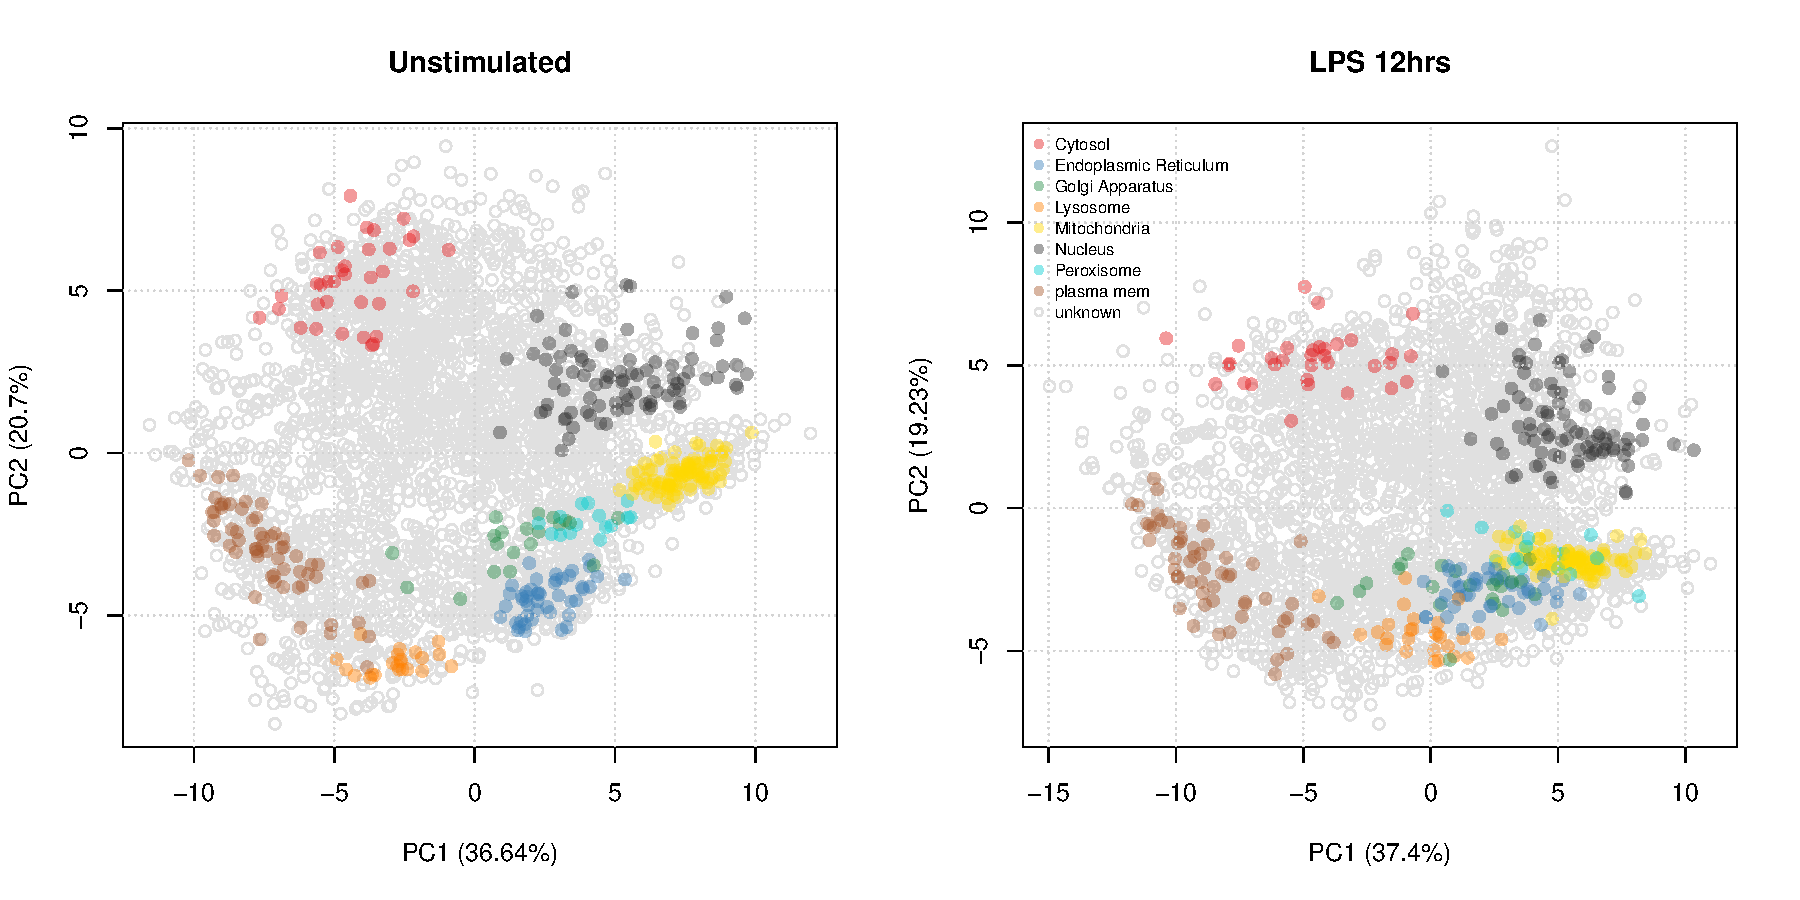
\includegraphics[width=\linewidth]{./figs_local/lps.pdf}
    \caption{Spatial maps of unstimulated and LPS-treated cells
      (combined triplicates).}
  \end{figure}
\end{frame}

\begin{frame}
  \begin{figure}[h]
    \centering
    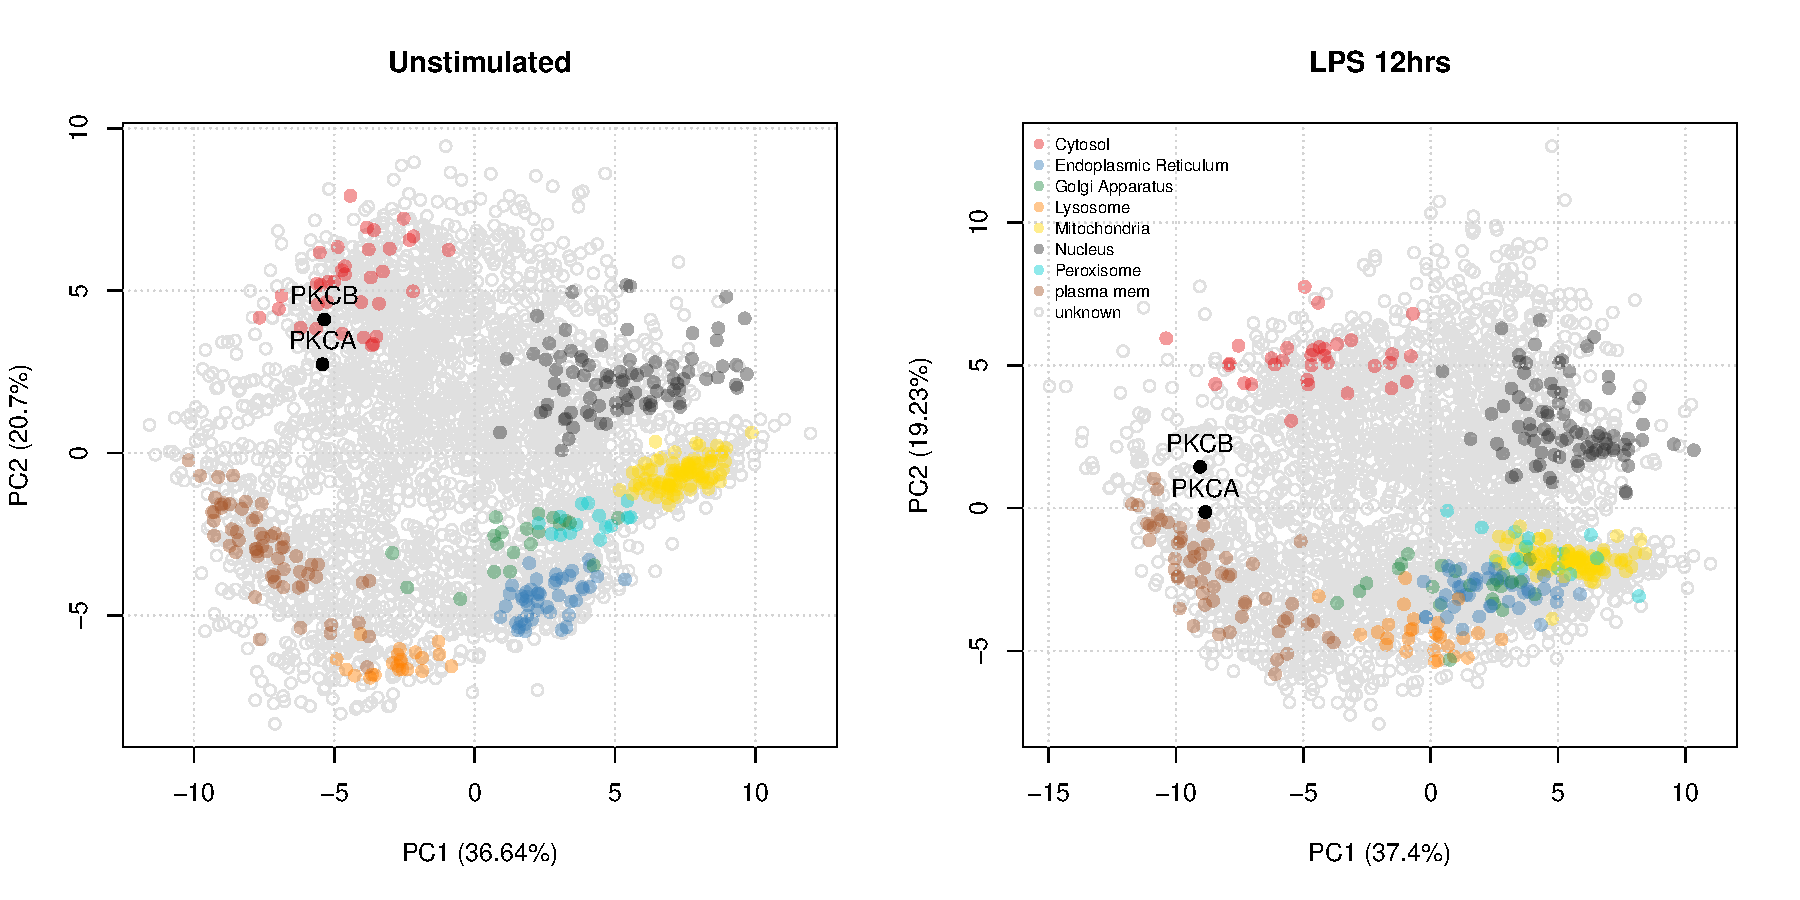
\includegraphics[width=\linewidth]{./figs_local/lps-pkc.pdf}
    \caption{Relocation of Protein Kinase C $\alpha$ and $\beta$ from the
      cytosol to the plasma membrane, \textbf{driving maturation into
        a differentiated macrophage phenotype}.}
  \end{figure}
\end{frame}

\begin{frame}
  \begin{figure}[h]
    \centering
    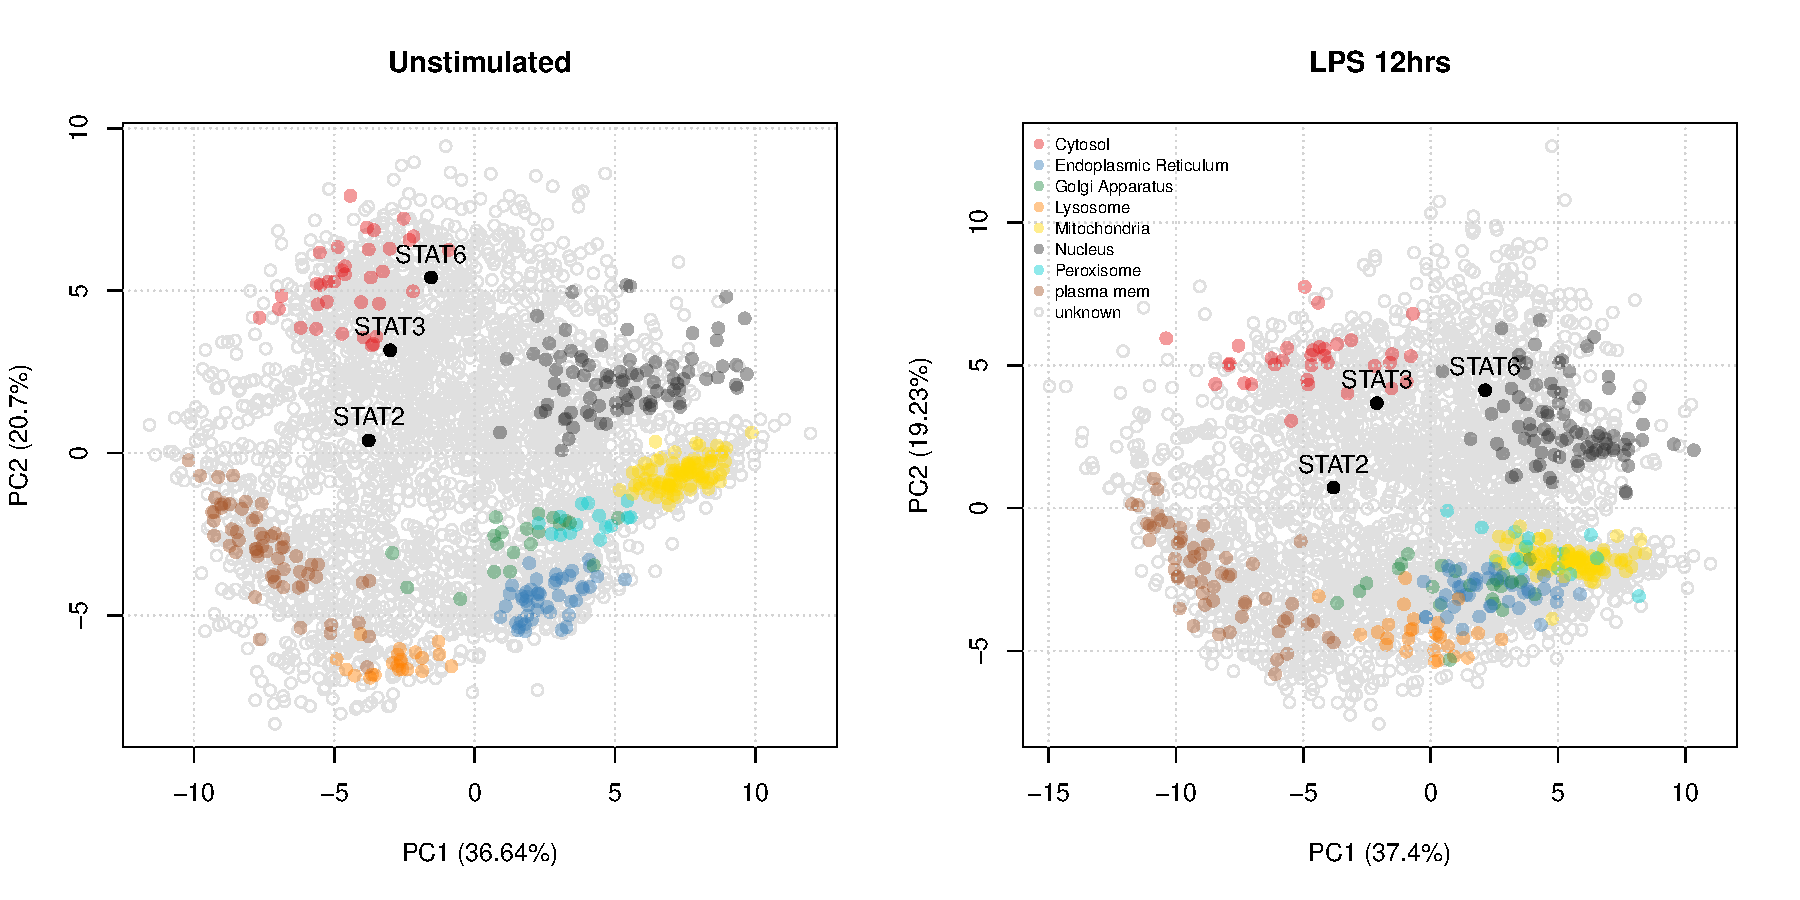
\includegraphics[width=\linewidth]{./figs_local/lps-stat.pdf}
    \caption{Relocation of Signal transducer and activator of
      transcription 6 (STAT6) from the cytosol to the Nucleus,
      \textbf{activating anti-bacterial and anti-viral-like
        response}. Validated by microscopy and see also
      \cite{Chen:2011}.}
  \end{figure}
\end{frame}
